\chapter{Methodology}

We will create our sound containing the data in a text file with the DosSend program. We will then read it back with DosRead and see how fast we can get back the former data.

\section{DosSend and DosRead usage}

\subsection{Using DosSend to create a wav file}

\subsubsection{Compiling the Program}

Compile the Java code using a Java compiler

\begin{lstlisting}
javac DosSend.java StdDraw.java
\end{lstlisting}

\subsubsection{Run the Program}

Run the compiled classes with Java and send it your data written in a .txt file.

\begin{lstlisting}
java DosSend.java < textfile.txt
\end{lstlisting}

\subsubsection{Output}

The program will convert the input text into an audio signal and save it as \texttt{DosOok\_message.wav}. It will also print characteristics of the signal to the console and display a graphical representation of the signal waveform.

\begin{figure}[!h]
	\begin{lstlisting}[style=console]
	[oli@oli-arch src]$ java DosSend < helloWorld.txt
	[ H e l l o   W o r l d   ! ]
	[ 1 0 1 0 1 0 1 0 0 0 0 1 0 0 1 0 1 0 1 0 0 1 1 0 0 0 1 1 0 1 1 0 0 0 1 1 0 1 1 0 1 1 1 1 0 1 1 0 0 0 0 0 0 1 0 0 1 1 1 0 1 0 1 0 1 1 1 1 0 1 1 0 0 1 0 0 1 1 1 0 0 0 1 1 0 1 1 0 0 0 1 0 0 1 1 0 0 0 0 0 0 1 0 0 1 0 0 0 0 1 0 0 ]
	Message : Hello World !
	Nombre de symboles : 13
	Nombre d'échantillons : 49392
	Durée : 1.12 s
	\end{lstlisting}
	\caption{Console output for the text "Hello World !"}
\end{figure}

\begin{figure}[!h]
	\begin{center}
		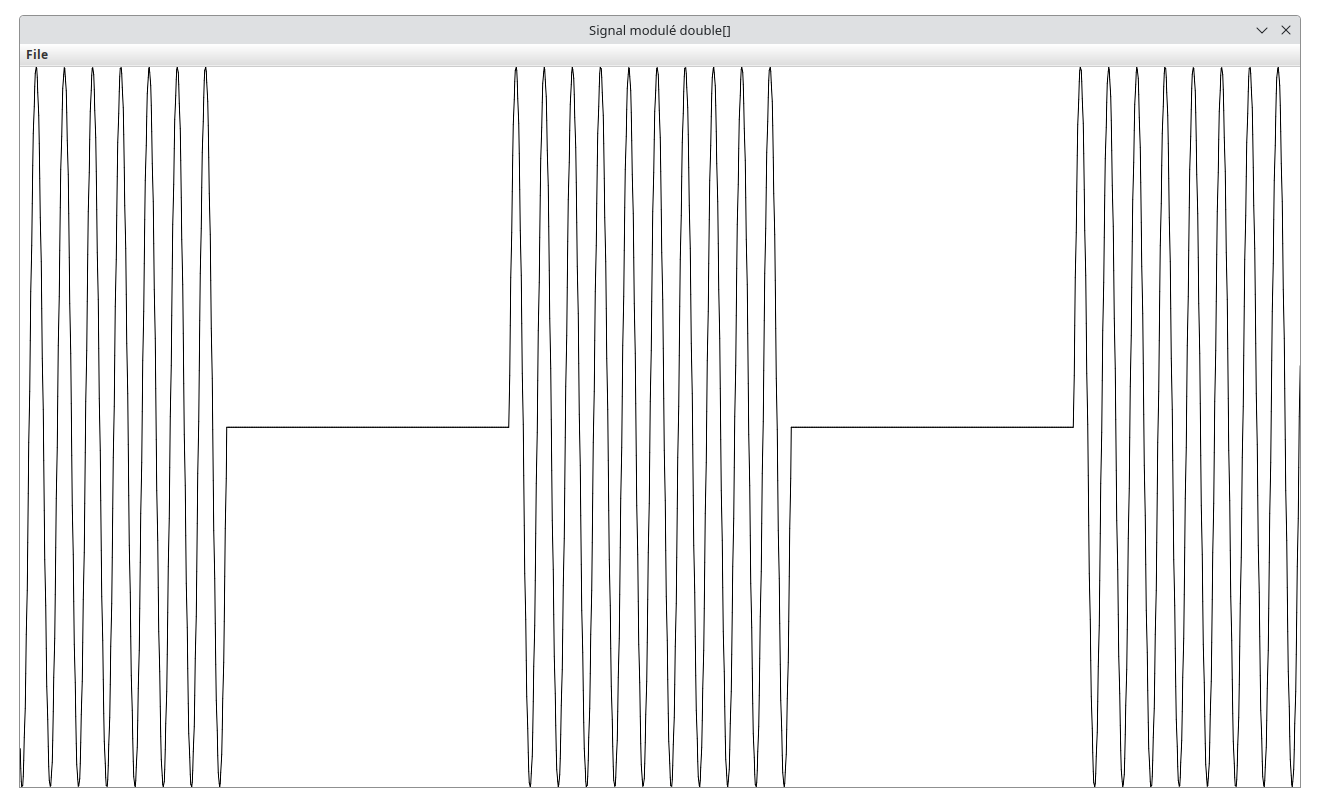
\includegraphics[width=15cm]{images/StdDraw1.png}
	\end{center}
	\caption{Signal output for the text "Hello World !" with start:300 stop:1000 mode:line}
\end{figure}

\subsection{Using DosRead}

\section{Monitoring the speed of the filter}

\section{Checking the filter's accuracy}